% !TeX spellcheck = en_GB
\section{\Duo}
The translation of \Duo{} \begin{CJK*}{UTF8}{bsmi}剁\end{CJK*}, referring to the cooking term \textit{to mince}, somehow suggests repetition and cutting using a part of the blade further away from the tip than \Pi{}. The movement itself is a combination of a forward extension with some sort of shearing, as if using a large cooking knife to mince herbs or vegetables.

In the \Yangjia{} \Michuan{} tradition, the emblematic \Duo{} is performed with both arms extended almost in line with the sword's blade (fig. \ref{fig:duo_full}). 


\begin{figure}[ht]
	\centering
	
	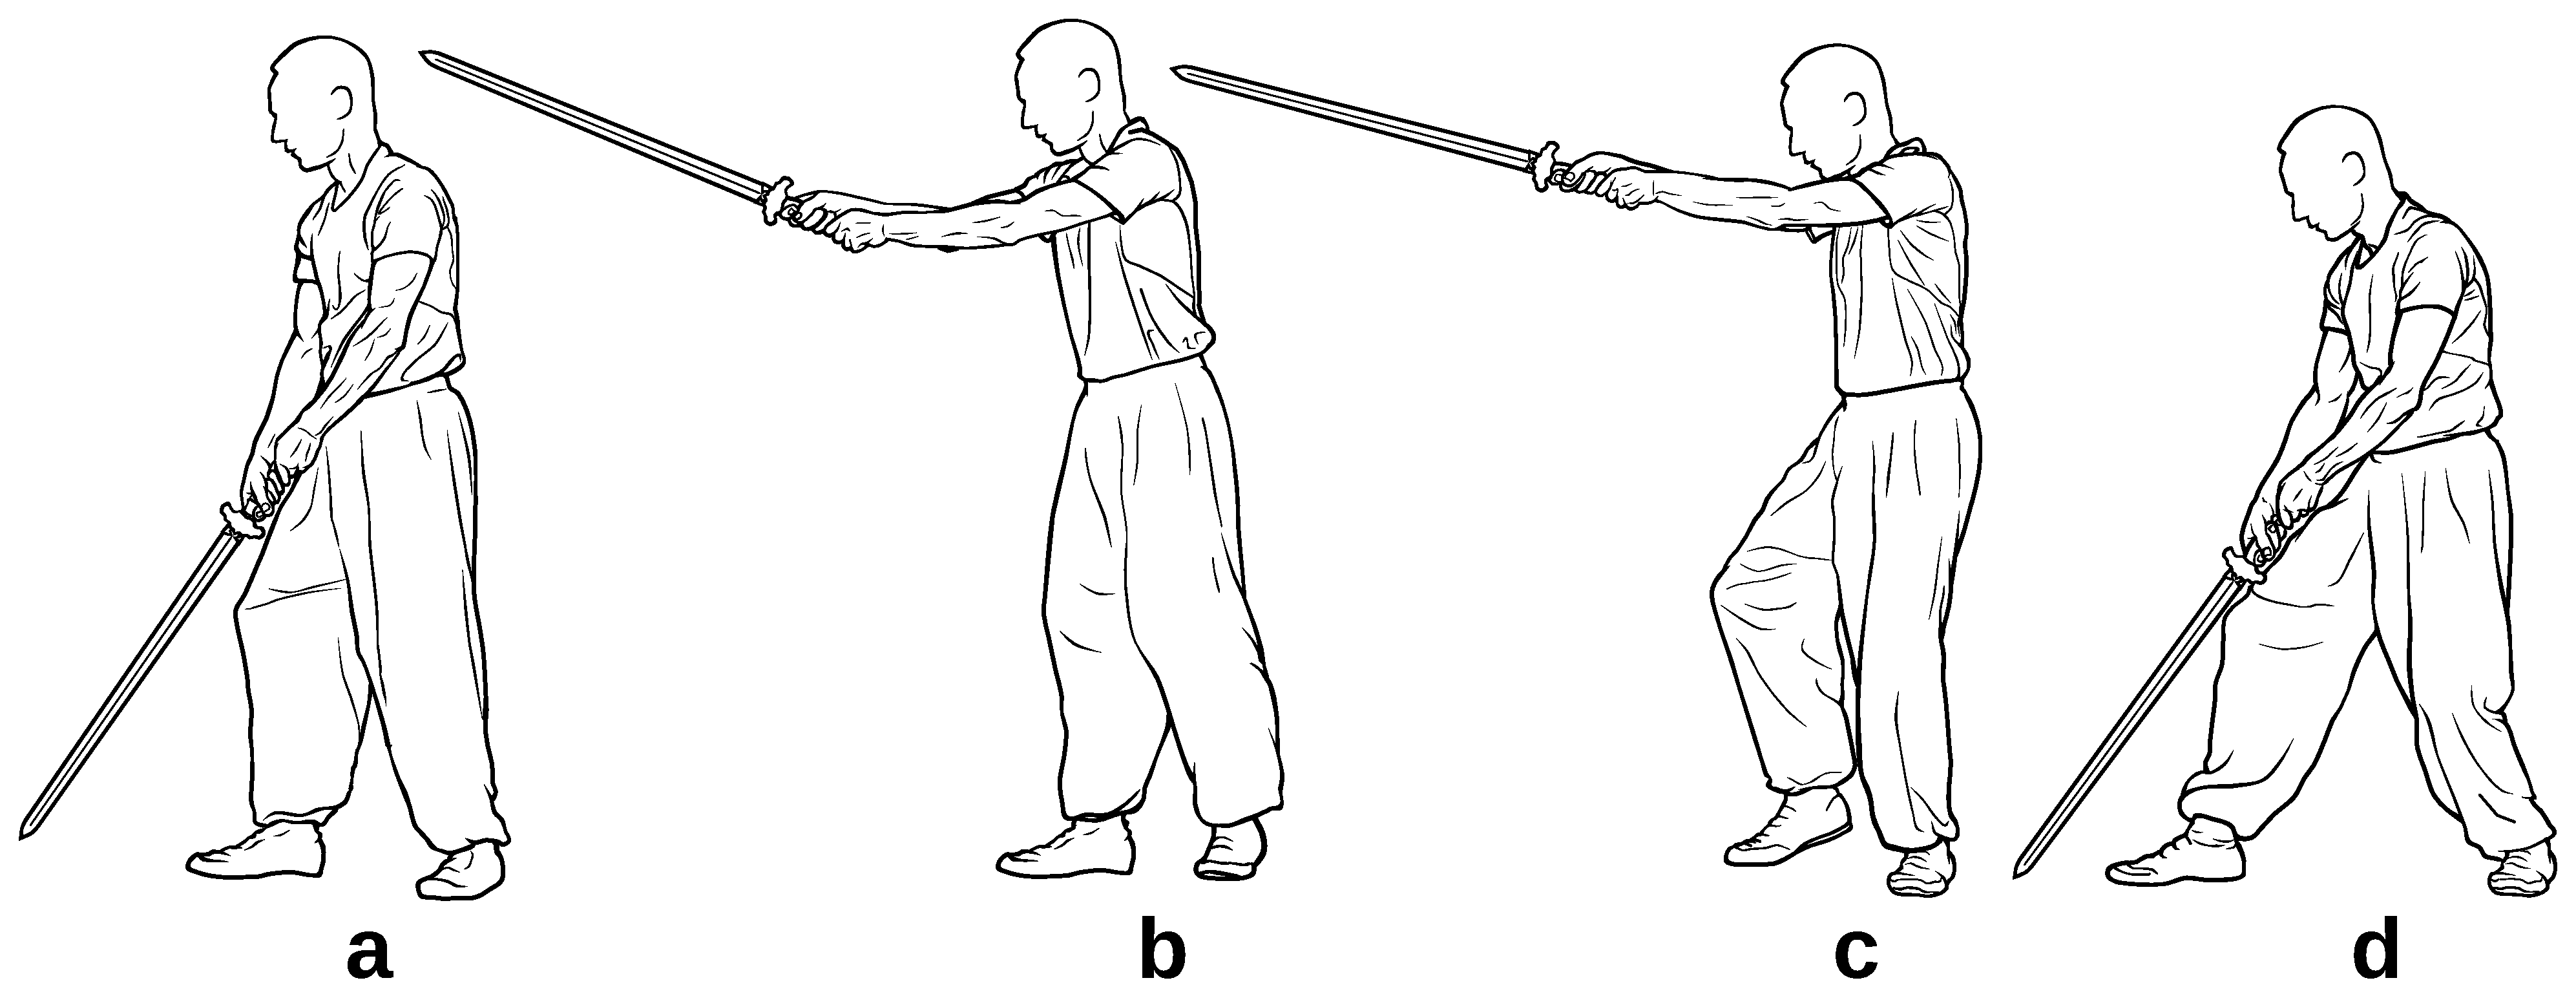
\includegraphics[width=1.00\textwidth]{../../Images/JibenJianfa/Duo/Duo.pdf}
	\caption[Advancing \Duo{}]{\Duo{} in the forward direction. From a low guard (a), raise the sword with a transfer of the weight onto the right foot (b), invert polarity and transfer the weight back onto the left foot (c), drop the sword while sinking in the left leg and advancing the right foot.}
	\label{fig:duo_full}
\end{figure} 

Even though both hands are in contact with the handle,  this should not be mistaken for a true double handed grip of the sword. While raising the sword and advancing, the right hand holds the sword while the left hand provides the structure and power coming from the waist by acting on the pommel along the direction of the blade. The combination of the right hand's passive role with the left hand's action creates a polarity resulting in a movement of the sword perpendicular to the axis of the right arm. When lowering the sword, the roles of both hands are inverted (fig. \ref{fig:duo_detail}). 

\begin{figure}[ht]
	\centering
	
	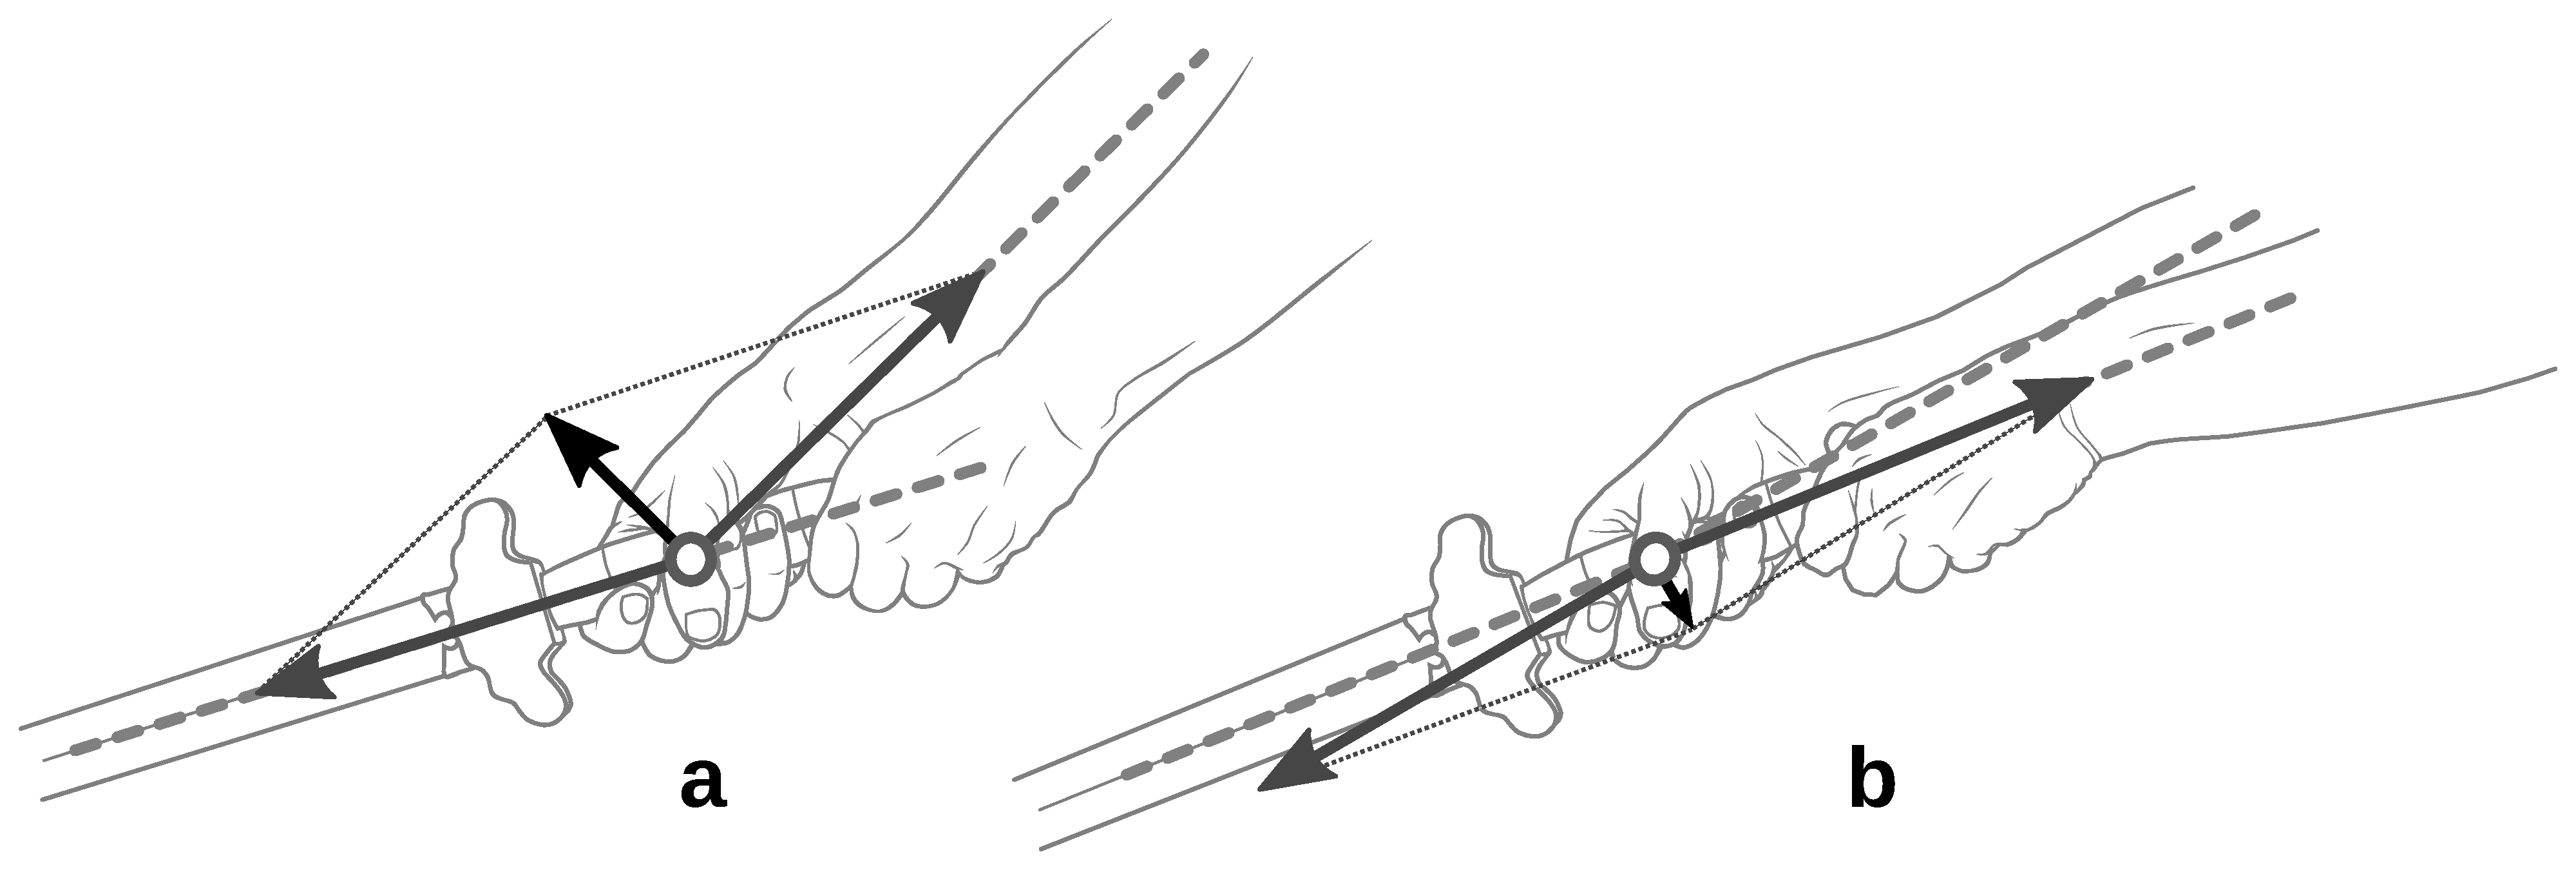
\includegraphics[width=1.00\textwidth]{../../Images/JibenJianfa/Duo/DuoDetail.pdf}
	\caption[Balance of forces in \Duo{}]{(a) To perform a forward rising \Duo{}, the left hand pushes the handle in the direction of the blade tip while the right arm passively balances the pushing force. Due to the angle between the pushing direction and the right arm, the resulting force perpendicular to the right arm pushes the sword upwards.\\
	(b) To perform a forward descending \Duo{}, the right hand pushes the handle while the left arm passively balances this force. The resulting force perpendicular to the left arm, draws the sword downwards.
	}
	\label{fig:duo_detail}
\end{figure} 

The power of the ascending forward \Duo{} thus originates in the weight transfer from the rear leg onto the fore leg, is transmitted to the sword by the left/rear hand with the right/fore hand exactly and passively balancing the forces to effortlessly generate the technique. An effective connexion between the waist and the sword will allow the explosive expression of the \Duo{} technique. 
This method somehow echoes the precepts found in the \JianJing{} stating that, when wielding a double-handed sword, power is first in the waist, then in the rear hand, and finally in the fore hand.

For the retreating \Duo{}, however, the hands play a reversed role: the right hand is active when raising the sword, and passive otherwise. As a rule of thumb, advancing or retreating, the active hand is always the one on the same side as the foot that is moving.

Since, when cooking, herbs are usually minced by cutting downwards, we may argue that the active phase of \Duo{} is the descending one. However, if we examine attentively the actual movement of a kitchen knife when mincing, we may discover that its form when cutting actually corresponds to the rising phase of \Duo{}. The main difference is that the tip of the knife stays down in contact with the table whereas the point of the sword rises up. But, in both cases, the edge follows the same movement relative to the tip. 
However, it is perfectly possible to be active in both phases, the actual passive phase being the transition movement between the ascending and descending parts of the technique. Thus, \Duo{} can be a raising thrust or cut as well as a descending cut, or, combined with \Mo{} energy, an action on the opponent's blade, either ascending to intercept and deflect or descending to shear. 

It is worth noting at this point that, since both hands are in contact with the hilt, the sword is always in line with the axis of the body. This axis is more to the left when we are on our left foot, in the low on-guard position that precedes the ascending forward phase of \Duo{}. Then, during the lifting phase of the movement, the axis is shifting to the right before being transferred back to the left when descending. Therefore, in the deflect/shear application of  \Duo{} in combination with \Mo{}, during the upward interception/deflection, transferring the weight onto the right/forward leg gently pushes the opponent's tip away, allowing the descending shear to naturally aim at the centre of the opponent's sword, deflecting it further to open the way for a hit while preventing any counter attack. 

\fiche{The simplest application of \Duo{} starts with a lower guard as an invitation for the opponent to prepare an attack. We can then engage and deflect with a \Duo{} before placing our riposte or we may take advantage of the explosive nature of the movement and use an offensive \Duo{} to thrust directly during the opponent's preparation.
\Duo{} is often performed in series of two to three movements, not more to avoid predictability, as seen for the double-handed version in the \Kunlun{} form. We can usually identify three periods in these series: The first \Duo{} movement would intercept an incoming attack, either a \Pi{} or a \Hua{} cut from above or a high level \Ci{} thrust.Then, the second one will deflect the opponent's blade to open the way for the third \Duo{} thrust. Of course, this is not a fixed pattern, and the first movement can be followed by any appropriate technique depending on the circumstances. For instance, instead of deflecting, the second step may accompany the opponent's blade to control it while entering to prepare the riposte.}

Although the classic movement is done with two hands, it is also possible to perform a \Duo{} with one hand only. In this case, the heel of the hand plays the same role as the rear hand in the two-handed version while the first three fingers \textemdash{} the index and middle fingers, and the thumb \textemdash{} play the part of the forehand (figure). 

During the ascending phase, the handle of the sword is pushed forwards by the heel of the hand and simultaneously pulled by the first three fingers. Given a good structure in the on-guard position, it is then possible, even with only one hand, to swiftly and effortlessly raise the sword from a low to a high position, for thrusting or engaging.  
\fiche{When descending, the fore fingers relax their grip while the ring and little fingers are tightened to pull the handle. Some intention should be put at the base of the index to gently push the handle downwards in the forward direction. The resulting structure allows to capture and deflect the centre of the opponent's sword by shearing or to perform a powerful cut while retreating.}
The alignment of the sword is quite similar to the two-handed version, with the tip of the blade in line with the body axis. However, the structure is not as strong as in the two-handed \Duo{} and, as a result, the shearing actions are not as powerful. However, this version of the movement is useful for quickly engaging the opponent's blade or a sudden attack from a lower guard. 

\fiche{
These actions can be chained, as in the \Kunlun{} sword form, by two or three, first intercepting the opponent's blade before deflecting and hitting with a double or treble shearing. 
the polarity between the hands allows the crossed links between hand and foot. 
}